% ============================================================
%  Curriculum Vitae — Rocélio da Silva
%  EN — Formal Executive: White, Black & Navy
% ============================================================
\documentclass[10pt,a4paper]{article}

\usepackage[utf8]{inputenc}
\usepackage[T1]{fontenc}
\usepackage[margin=0pt]{geometry}
\usepackage{array,tabularx}
\usepackage{enumitem}
\usepackage{hyperref}
\usepackage{xcolor}
\usepackage{graphicx}
\usepackage{tikz}
\usepackage{setspace}
\usepackage{parskip}
\usepackage{amssymb}

\usetikzlibrary{calc}

% ============================================================
%  COLOURS — Formal white document
% ============================================================
\definecolor{navy}{HTML}{1A3A5C}
\definecolor{navylt}{HTML}{2E5F8A}
\definecolor{goldrule}{HTML}{C8A84B}
\definecolor{bodytext}{HTML}{1A1A1A}
\definecolor{mutedtext}{HTML}{555555}
\definecolor{sidetext}{HTML}{EEF4FA}
\definecolor{sidebg}{HTML}{1A3A5C}

% ============================================================
%  GLOBAL
% ============================================================
\color{bodytext}
\pagestyle{empty}
\setlength{\parindent}{0pt}
\setlength{\parskip}{2pt}

\hypersetup{colorlinks=true, urlcolor=navylt, linkcolor=navylt}

% ============================================================
%  SIDEBAR SECTION
% ============================================================
\newcommand{\sideSection}[1]{%
  \vspace{2pt}%
  {\bfseries\color{sidetext}\small\MakeUppercase{#1}}%
  \par\vspace{1pt}%
  {\color{goldrule}\rule{\linewidth}{0.55pt}}%
  \par\vspace{1pt}%
}

% ============================================================
%  MAIN SECTION
% ============================================================
\newcommand{\mainSection}[1]{%
  \vspace{1pt}%
  {\bfseries\color{navy}\large\MakeUppercase{#1}}%
  \par\vspace{0pt}%
  {\color{navy}\rule{\linewidth}{1.0pt}}%
  \par\vspace{1pt}%
}

% ============================================================
%  EXPERIENCE ENTRY
% ============================================================
\newcommand{\expEntry}[3]{%
  {\bfseries\color{navy}\normalsize #1}\par\vspace{1pt}%
  {\color{mutedtext}\small #2 \hfill \textit{\color{navylt}#3}}\par\vspace{1pt}%
}

% ============================================================
%  LISTS
% ============================================================
\setlist[itemize]{
  itemsep=0pt,
  topsep=0pt,
  leftmargin=1.3em,
  label={\color{navylt}\small$\bullet$}
}

\begin{document}

% ============================================================
%  SIDEBAR BACKGROUND
% ============================================================
\noindent
\begin{tikzpicture}[remember picture, overlay]
  \fill[sidebg]
    (current page.north west)
    rectangle
    ([xshift=0.295\paperwidth] current page.south west);
  \draw[goldrule, line width=1.0pt]
    ([xshift=0.295\paperwidth] current page.north west)
    -- ([xshift=0.295\paperwidth] current page.south west);
\end{tikzpicture}

% ============================================================
%  LEFT SIDEBAR
% ============================================================
\noindent
\begin{minipage}[t]{0.283\paperwidth}
  \color{sidetext}
  \setlength{\parskip}{3pt}
  \hspace*{10pt}%
  \begin{minipage}[t]{\dimexpr\linewidth-18pt}

    \vspace{5pt}
    \begin{center}
      \IfFileExists{photo.png}{%
        \begin{tikzpicture}
          \clip (0,0) circle (0.72in);
          \node[inner sep=0pt] at (0,0)
            {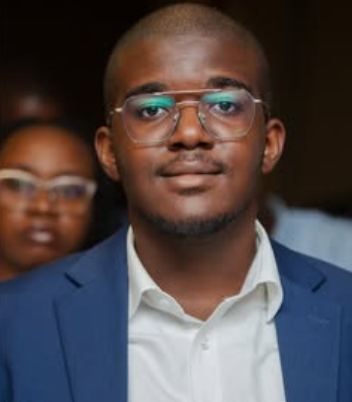
\includegraphics[width=1.44in,height=1.44in,keepaspectratio]{photo.png}};
          \draw[white, line width=2pt] (0,0) circle (0.72in);
        \end{tikzpicture}%
      }{%
        
\begin{tikzpicture}
          \fill[white] (0,0) circle (0.72in);
          \draw[goldrule, line width=1.6pt] (0,0) circle (0.72in);
          \node[font=\bfseries\LARGE, text=navy] at (0,0) {RS};
        \end{tikzpicture}%
      }
      \par\vspace{2pt}
      {\large\bfseries\color{white} Rocélio da Silva}\par\vspace{2pt}
      {\small\color{sidetext!80} Offshore \& Engenharia Upstream}\par\vspace{2pt}
      {\color{goldrule}\rule{0.70\linewidth}{0.5pt}}
    \end{center}

    \sideSection{Contacto}
    {\small
      \textbf{\color{white}Tel\,} \color{sidetext}+244 924 010 222\par\vspace{2pt}
      \textbf{\color{white}Email\,} \href{mailto:rocelioinc@gmail.com}{\color{goldrule!80}rocelioinc@gmail.com}\par\vspace{2pt}
      \textbf{\color{white}Local\,} \color{sidetext}Benfica, Luanda\par
    }

    \sideSection{Formação}
    {\small
      \textbf{\color{white}ISPTEC}\par
      \color{sidetext}Lic.\  Eng.\ de Petróleos\par
      \textit{\color{goldrule!80}2022 -- Presente $\cdot$ 3.º Ano}\par\vspace{2pt}
      \textbf{\color{white}CEPI}\par
      \color{sidetext}Diploma do Ensino Secundário\par
      \textit{\color{goldrule!80}2020 -- 2022}\par
    }

    \sideSection{Línguas}
    {\small
      \begin{tabular}{@{}l@{\hspace{6pt}}r@{}}
        \textbf{\color{white}Português} & \color{sidetext}Nativo \\[3pt]
        \textbf{\color{white}Inglês}    & \color{goldrule!90}TOEFL 99 \\
      \end{tabular}
    }

    \sideSection{Competências Técnicas}
    {\small
      \begin{itemize}[leftmargin=1em,
                      label={\color{goldrule}\tiny$\blacktriangleright$},
                      itemsep=0pt, topsep=1pt]
        \item \color{sidetext}Python -- Pandas, Matplotlib
        \item \color{sidetext}Calc.\ Factor Z (Pitzer, Papay)
        \item \color{sidetext}Selecção de Métodos EOR
        \item \color{sidetext}Reservatórios \& Poços
        \item \color{sidetext}Fluidos de Perfuração Offshore
        \item \color{sidetext}GIS básico $\cdot$ Blender 3-D
        \item \color{sidetext}C,\; HTML / CSS
      \end{itemize}
    }

    \sideSection{Liderança}
    {\small
      \begin{itemize}[leftmargin=1em,
                      label={\color{goldrule}\tiny$\blacktriangleright$},
                      itemsep=0pt, topsep=1pt]
        \item \color{sidetext}Presidente de Membros
        \item \color{sidetext}Gestão de Eventos
        \item \color{sidetext}Comunicação Técnica
        \item \color{sidetext}Trabalho em Equipa
      \end{itemize}
    }

    \sideSection{Afiliações}
    {\small
      \textbf{\color{white}SPE} \color{sidetext}-- Soc.\ de Eng.\ de Petróleos\par
      \textit{\color{goldrule!80}Membro Estudantil}\par\vspace{2pt}
      \textbf{\color{white}MIT Global Classroom}\par
      \textit{\color{goldrule!80}Participante, 2025}\par
    }

    \vspace{4pt}
    \begin{center}
      {\color{goldrule}\rule{0.55\linewidth}{0.4pt}}\par\vspace{2pt}
      {\color{sidetext!60}\small\itshape Referências a pedido}
    \end{center}

  \end{minipage}
\end{minipage}%
%
% ============================================================
%  RIGHT — MAIN CONTENT  (white background, dark text)
% ============================================================
\hspace*{10pt}%
\begin{minipage}[t]{\dimexpr 0.705\paperwidth - 26pt}
  \color{bodytext}
  \setlength{\parskip}{2pt}
  \setstretch{1.00}

  \vspace{5pt}

  % ---- NAME HEADER ----
  {\huge\bfseries\color{navy} ROCÉLIO DA SILVA}\par
  \vspace{2pt}
  {\normalsize\color{mutedtext}
    Offshore \& Engenharia Upstream
    $\cdot$ Membro SPE
    $\cdot$ Luanda, Angola
  }\par
  \vspace{2pt}
  {\color{navy}\rule{\linewidth}{1.2pt}}\par
  \vspace{1pt}
  {\color{goldrule}\rule{\linewidth}{0.4pt}}

  % ---- PROFILE ----
  \mainSection{Perfil}
  \setstretch{1.00}
  Estudante do 3.º ano de Engenharia de Petróleos no ISPTEC com forte vocação para
  operações \textbf{offshore} e desenvolvimento de software técnico para a indústria
  petrolífera. Líder da equipa ISPTEC no PetroChamp, Presidente de Membros do SPE
  Student Chapter e participante do MIT Global Classroom (2025). Desenvolve ferramentas
  Python para cálculos de engenharia de reservatórios (factor Z, EOR). Fluente em
  Inglês (TOEFL~99) e comprometido com excelência técnica em mercados emergentes.
  \setstretch{1.00}

  % ---- PROFESSIONAL EXPERIENCE ----
  \mainSection{Experiência Profissional}

  \expEntry{Presidente de Membros -- SPE Student Chapter}%
           {ISPTEC / Society of Petroleum Engineers}%
           {2026 -- Presente}
  \begin{itemize}
    \item Lidera o recrutamento, envolvimento e retenção de membros.
    \item Coordena seminários técnicos e promove ligações entre estudantes e a indústria.
  \end{itemize}

  \vspace{2pt}
  \expEntry{Secretário de Assuntos Académicos}%
           {AEISPTEC -- Associação de Estudantes do ISPTEC}%
           {2025}
  \begin{itemize}
    \item Coordenou eventos académicos e actividades departamentais.
    \item Geriu comunicações e documentação académica dos estudantes.
    \item Serviu de elo de ligação entre a liderança académica e o corpo estudantil.
  \end{itemize}

  % ---- KEY PROJECTS ----
  \mainSection{Projectos-Chave}

  {\small\bfseries\color{navy}Estudo de Viabilidade Solar Comunitária -- MIT--ISPTEC (2025)}\par
  {\footnotesize\color{mutedtext}MIT Global Classroom $\cdot$ Iniciativa de Acesso à Energia em Angola}
  \begin{itemize}
    \item Selecção de locais óptimos via análise GIS e modelagem de procura energética.
    \item Apresentou resultados a parceiros internacionais e à liderança do ISPTEC.
    \item Impacto directo na estratégia de acesso à energia para comunidades desfavorecidas em Angola.
  \end{itemize}

  \vspace{2pt}
  {\small\bfseries\color{navy}Calculadora Factor Z \& Ferramenta EOR -- Python (2024--2025)}\par
  {\footnotesize\color{mutedtext}Engenharia de Software $\cdot$ ISPTEC}
  \begin{itemize}
    \item Calculadora Python do factor Z (Pitzer--Curl, Papay) para condições de reservatório.
    \item Módulo de selecção de método EOR: análise multicritério (WAG, polímeros,
          CO\textsubscript{2} flooding).
    \item CLI interactiva; exportação CSV e gráficos Matplotlib.
  \end{itemize}

  % ---- ACHIEVEMENTS ----
  \mainSection{Conquistas \& Reconhecimento}

  \renewcommand{\arraystretch}{1.40}
  \begin{tabular}{@{} p{0.06\linewidth} p{0.88\linewidth} @{}}
    {\footnotesize\bfseries\color{navy}2025} &
      \textbf{PetroChamp -- Líder de Equipa ISPTEC:} Liderou a equipa ISPTEC
      na competição técnica PetroChamp, demonstrando excelência académica e
      liderança sob pressão.\\
    {\footnotesize\bfseries\color{navy}2025} &
      \textbf{Orador \& Anfitrião} -- Semana Académica de Geociências (ISPTEC);
      coordenou oradores multinacionais.\\
    {\footnotesize\bfseries\color{navy}2025} &
      \textbf{MIT Global Classroom} -- Solar Comunitário em Angola; estudo
      apresentado a colaboradores internacionais.\\
    {\footnotesize\bfseries\color{navy}2022} &
      \textbf{TOEFL 99/120} -- Proficiência avançada em Inglês; habilitou
      colaborações SPE e MIT.\\
  \end{tabular}
  \renewcommand{\arraystretch}{1}

  % ---- CAREER OBJECTIVES ----
  \mainSection{Objectivos de Carreira}
  \setstretch{1.00}
  Procuro uma posição em \textbf{operações offshore} ou upstream onde possa combinar
  competências em engenharia de reservatórios, desenvolvimento de software técnico
  (Python) e liderança de equipas para contribuir para operações eficientes e
  sustentáveis em Angola e na África Subsariana.
  \setstretch{1.00}

  \vspace{2pt}
  {\color{navy}\rule{\linewidth}{0.8pt}}\par
  \vspace{1pt}
  {\color{goldrule}\rule{\linewidth}{0.4pt}}\par
  \vspace{2pt}
  {\footnotesize\color{mutedtext}\itshape
    Engenharia de Petróleos $\cdot$ Angola $\cdot$ 2025}

\end{minipage}

\end{document}
